\chapter{Data Compression}

The previous two chapters described the process of turning an analog information signal into a digital sequence using sampling and quantization.
From here on, we assume that information sources are digital in nature.
That is, they produce a succession of symbols, each drawn from a \emph{discrete alphabet}.
The two main goals of the current chapter are to find an adequate measure of information for digital systems and to describe compression algorithms that can be employed to represent the said information in a succinct manner.
\emph{Data compression}, also known as \emph{source coding}, is important because it reduces the consumption of expensive resources such as hard disk space or transmission bandwidth.
Alternatively, it can be applied to lower the cost of communication, reduce latency or improve the quality of the received messages.

This document provides an introduction to \emph{lossless compression} algorithms, whereby the original message can be recovered perfectly from the compressed data.
This is in contrast with \emph{lossy data compression}, which can achieve much better compression ratio at the expense of introducing some distortion in the message.
In the latter case, part of the information is lost and the original data cannot be recovered perfectly, although the reconstructed message may be quite close to the original one.
For instance, the JPEG algorithm can be employed as a lossy compression scheme to reduce the size of a digital photograph.
In lossless data compression, two strategies are employed to reduce the expected size of a message.
First, highly probable symbols are assigned short descriptions, and less likely symbols are then necessarily encoded using longer codewords.
Second, the statistical redundancy contained in the input signal is removed, leading to a more concise representation of the digital data.
Two lossless compression algorithms are explained more thoroughly below.

As we will see, finding a pertinent measure of information is essential in assessing the performance and limitations of compression algorithms.
While the general notion of information may be quite broad, it has a precise definition in the context of digital communication systems.
To describe this specific meaning, we need to develop a rigorous mathematical model for digital information sources.


\section{Discrete Memoryless Sources}

As mentioned above, a digital source produces a sequence of symbols drawn from a countable alphabet.
It can therefore be modeled as a discrete-time random process.
Because of their indeterminate nature, random signals and stochastic processes can be quite hard to characterize.
In Section~\ref{section:StocahsticSignalsFAS}, we introduced two desirable attributes of random signals, namely stationary and ergodicity.
Yet we purposely avoided giving an explicit definition for a random process.
A detailed treatment of the subject requires advanced concepts from probability theory, a topic that interested readers may wish to pursue on their own.
For the sake of simplicity, we only consider elementary information sources in this document.
These sources are collectively known as discrete memoryless sources.
They are easy to analyze and can be described unambiguously in a straightforward manner.
Furthermore, discrete memoryless sources provide valuable insights into the design of efficient compression algorithms.

\begin{definition}
A \emph{discrete memoryless source} is a digital information source that produces a sequence of independent and identically distributed symbols over time.
Mathematically, it consists of an alphabet $\mathcal{X}$ and a probability mass function $p_X(\cdot)$ such that, at any time~$t$, the probability that the source outputs symbol $x \in \mathcal{X}$ is equal to $p_X(x)$.
\end{definition}

We stress that, for discrete memoryless sources, it suffices to define the probability mass function of individual symbols to completely characterize the statistical properties of the corresponding random signal.
The higher-order statistics need not be specified explicitly, as they can be obtained using
\begin{equation} \label{equation:JointDistributionMemorylessSource}
\Pr (X_{t_1} = x_{t_1}, \ldots, X_{t_n} = x_{t_n})
= p_X(x_{t_1})  \cdots p_X(x_{t_n})
\end{equation}
where $x_{t_1}, \ldots, x_{t_n} \in \mathcal{X}$.
In \eqref{equation:JointDistributionMemorylessSource}, the random variable $X_{t_i}$ denotes the output of the source at time~$t_i$.

From a intuitive point of view, the information rate of a discrete memoryless source should be equal to the amount of information it produces at every time instant.
In other words, the amount of information created by a discrete memoryless source $X$ at time~$t$ should be computable based on $\mathcal{X}$ and $p_X(\cdot)$, exclusively.
We provide two examples of memoryless sources below to further illustrate their form.

\begin{example}[Binary Source] \label{example:BinarySource}
The simplest possible information source is a discrete memoryless source where $p_X(\cdot)$ is the probability mass function of a Bernoulli random variable,
\begin{equation*}
p(x) = \begin{cases} (1 - p), & x = 0 \\
p, & x = 1 \end{cases}
\end{equation*}
with $p \in [0,1]$.
For instance, this source can be employed to model the successive flipping of a biased coin where heads is obtained with probability $p$ and tails is obtained with probability $1 - p$.
\end{example}

\begin{example}
To produce a slightly more elaborate example, consider a collection of experiments where a fair coin is flipped repetitively until heads is observed.
The outcome of each experiment is reported as a source output.
The source alphabet in this case is $\mathcal{X} = \{1, 2, \ldots \}$ and the marginal probability mass function associated with individual outcomes becomes
\begin{equation*}
p_X (x) = \frac{1}{2^x}, \quad x = 1, 2, \ldots
\end{equation*}
Thus, the distribution of the source output at time~$t$ is a geometric random variable with parameter $p = \frac{1}{2}$.
\end{example}

It is straightforward to show that all discrete memoryless sources are both stationary and ergodic.
The fact that their outcomes are independent through time makes them convenient for analysis, leading to simpler interpretations.
However, it should also be pointed out that many realistic sources are much more complicated than memoryless sources.
In particular, they may be correlated through time, which will have a major impact on their information rates.
Handling complex sources require heavier mathematical machinery, and is beyond the scope of this document.
Having constructed a suitable abstraction for information sources, we are now ready to discuss entropy, a concept closely related to the notion of information.


\section{Entropy}

The \emph{entropy} can be viewed as a measure of uncertainty in a random variable.
In the context of digital communications, it serves as a measure of information in that it provides a lower bound on the expected number of bits required to describe the output of a discrete memoryless source.
This lower bound is tight and can be approached using different schemes, as we will see shortly.

\begin{definition}[Entropy]
Let $X$ be a discrete random variable drawn from alphabet $\mathcal{X}$ according to probability mass function $p_X(\cdot)$.
The entropy of $X$, denoted $H(X)$, is defined by
\begin{equation} \label{equation:Entropy}
H(X) = - \sum_{x \in \mathcal{X}} p_X (x) \log_2 ( p_X(x) ) .
\end{equation}
Under our definition, entropy is described in bits.
When writing $H(X)$, we use the convention
\begin{equation*}
0 \log_2 \left( \frac{1}{0} \right)
= \lim_{\epsilon \rightarrow 0} \epsilon \log_2 \left( \frac{1}{\epsilon} \right)
= 0 .
\end{equation*}
Alternatively, the entropy of $X$ can be interpreted as an expected value
\begin{equation*}
H(X) = \mathrm{E} \left[ \log_2 \left( \frac{1}{p_X(X)} \right) \right] .
\end{equation*}
\end{definition}

\begin{example} \label{example:EntropyFairCoin}
Let $X$ be an abstract representation of the flipping of a fair coin.
The probability mass function of $X$ is then
\begin{equation*}
p(x) = \begin{cases} 0.5, & x = 0 \\
0.5, & x = 1 \end{cases}
\end{equation*}
with zero representing tails and one denoting heads.
We can compute the entropy of $X$ as follows,
\begin{equation*}
H(X) = - \frac{1}{2} \log_2 \left( \frac{1}{2} \right)
- \frac{1}{2} \log_2 \left( \frac{1}{2} \right) = 1 \text{ bit.}
\end{equation*}
Hence, the minimum expected number of bits needed to describe the outcome of a coin toss is one; this seems reasonably intuitive.
\end{example}

The entropy as defined in \eqref{equation:Entropy} has interesting properties.
The function $H(X)$ does not depend on the actual symbols themselves, it only depends on the probability mass function of the possible outcomes.
For the flipping of a coin in Example~\ref{example:EntropyFairCoin}, the entropy of $X$ remains the same whether we represent tails by a zero or a string of letters.
More generally, the way we choose to designate the outcomes of a random experiment has no impact over the entropy of the corresponding source, only the relative probabilities of the symbols matter.

The entropy of pair of two independent random variables is the sum of the individual entropy.
Suppose that $X$ is a vector random variable given by $X = (V_1, V_2)$ where $V_1$ and $V_2$ are independent.
Then $p_X(x) = p_X((v_1, v_2)) = p_{V_1} (v_1) p_{V_2} (v_2)$ and
\begin{equation*}
\begin{split}
H(X) &= - \sum_{ x \in \mathcal{X} } p_X(x) \log_2 \left( \frac{1}{p_X(x)} \right) \\
&= - \sum_{(v_1, v_2) \in \mathcal{V}_1 \times \mathcal{V}_2}
p_X((v_1, v_2)) \log_2 \left( \frac{1}{p_X((v_1, v_2))} \right) \\
&= - \sum_{v_1 \in \mathcal{V}_1} \sum_{v_2 \in \mathcal{V}_2}
p_{V_1} (v_1) p_{V_2} (v_2) \log_2 \left( \frac{1}{p_{V_1} (v_1) p_{V_2} (v_2)} \right) \\
&= - \sum_{v_1 \in \mathcal{V}_1}
p_{V_1} (v_1) \log_2 \left( \frac{1}{p_{V_1} (v_1)} \right)
- \sum_{v_2 \in \mathcal{V}_2}
p_{V_2} (v_2) \log_2 \left( \frac{1}{p_{V_2} (v_2)} \right) \\
&= H(V_1) + H(V_2) .
\end{split}
\end{equation*}
This corresponds to our intuitive understanding of information.
The amount of information contained in two unrelated events should be the sum of the information contained in each individual event.

It is important to emphasize that $H(X)$ is computed based on the distribution $p_X(\cdot)$; it is not a function of the random variable $X$ itself.
As such, $H(X)$ is a deterministic quantity and does not depend on the actual realization of $X$.
Furthermore, we note that $H(X)$ is continuous in the weights of the distribution $p_X(\cdot)$.
A small change in the probability mass function of $X$ only results in a small variation in its entropy.
It is therefore possible to construct accurate entropy estimates based on empirical measurements of the source outputs.


\section{Source Codes}

A compression code is a rule for converting a symbol (or a group of symbols) into a string of bits called a codeword.
The goal of the code, of course, is to provide a more concise representation of the information signal.
Mathematically, an encoder is a function $c : \mathcal{X} \mapsto \mathcal{C}$ from the input alphabet $\mathcal{X}$ to the collection of possible codewords $\mathcal{C}$.
In lossless compression, the function $c$ must be injective over the support of $X$; without this one-to-one relationship, decoding errors are bound to happen.

Encoding schemes can be partitioned into two categories based on the structure of their codebooks.
If the codewords all share the same bit-length, then the corresponding code is called a \emph{fixed-length code}.
Such codes are easy to encode and decode, yielding unambiguous messages.
However, they cannot be used to compress data by assigning short descriptions to most frequent symbols and longer descriptions to the less likely ones.
Data compression in fixed-length coding methods is only possible for large blocks of data, and any compression beyond the logarithm of the total number of possibilities comes with a finite, though perhaps small, probability of decoding failure.

Lossless data compression systems often employ variable-length codes.
As the name suggests, a \emph{variable-length code} is an encoding function that maps source symbols to a variable number of bits.
This is a suitable feature for many compression schemes as the greater flexibility leads to better compression ratio.
However, in dealing with variable-length codes, it is essential to recognize that they can be more tricky.
For instance, it is impossible to know where codewords begin in a binary file without looking at the content of the file.
This is in stark contrast with fixed-length codes where codewords are positioned at regular intervals.
To ensure that the binary output of a variable-length encoder can be recovered unambiguously, the code needs specific properties.

Variable-length codes can be nested in order of decreasing generality as non-singular, uniquely decodable and instantaneous.
A code is \emph{non-singular} if each source symbol is mapped to a different bit string.
That is, the mapping $c$ from $\mathcal{X}$ to $\mathcal{C}$ is one-to-one.
In contrast, if two symbols map to the same codeword then it is intuitively clear that the original message cannot be recovered.

A code is \emph{uniquely decodable} if its extensions are non-singular.
The extension of a code $c$ is obtained by concatenating its codewords when $c$ is applied to the cartesian product $\mathcal{X}^n$; it can be expressed as
\begin{equation*}
c^{(n)} (x_1, \ldots, x_n) = c(x_1) \cdots c(x_n)
\end{equation*}
where $n$ is an integer.
Note that an extension of $c$ is a proper encoding schemes because it takes a group of symbols as its input and produces a string of bits as its output.

Finally, a code is \emph{instantaneous} if no codeword in $\mathcal{C}$ is a prefix of a different encoded symbol under the mapping $c$.
An instantaneous code is also called a \emph{prefix code} because it satisfies the prefix condition: no codeword is a prefix of any other codeword in $\mathcal{C}$.
This property implies that received symbols can be decoded immediately after their entire codeword is received or read.
Furthermore, a message con be transmitted as a sequence of concatenated code words without markers to frame the words in the message.

\begin{example}
Suppose that a source produces three possible symbols, $\mathcal{X} = \{ x_1, x_2, x_3 \}$.
We consider four codes ($c_1, c_2, c_3, c_4$) with different properties.
The encoding schemes are defined as follows,
\begin{center}
\begin{tabular}{|c|c|c|c|c|}
\hline
Source Symbol & \multicolumn{4}{c|}{Codeword} \\
\hline
$x$ & $c_1(x)$ & $c_2(x)$ & $c_3(x)$ & $c_4(x)$ \\
\hline
$x_1$ & 0 & 0 & 0 & 0 \\
$x_2$ & 1 & 1 & 01 & 10 \\
$x_3$ & 0 & 01 & 11 & 11 \\
\hline
\end{tabular} .
\end{center}
The first scheme is not injective as it maps different source symbols to the same codeword, $c_1(x_1) = c_1(x_3)$.
Thus, individual codewords cannot be decoded unambiguously.
The second code is one-to-one, however it is not uniquely decodable.
The encoded message 01 can be generated by either input string $x_1 x_2$ or input symbol $x_3$.
Clearly, the compressed message cannot be decoded unambiguously.
The third code, $c_3(\cdot)$ is uniquely decodable, but not instantaneous.
While $c_4(\cdot)$ is a prefix code where every symbol can be decoded immediately after reception.
\end{example}

The measure of a good prefix code is the expected length of its encoded symbols.
Suppose that a discrete memoryless source $(\mathcal{X}, p_X)$ is given along with a code $c$.
We denote the length of codeword $c(x)$ by $l_c(x)$.
The expected number of bits produced by the source at each time instant is then given by
\begin{equation} \label{equation:CodeRateCompression}
\mathrm{E} [ l_c (X) ] = \sum_{x \in \mathcal{X}} p_X(x) l_c(x) .
\end{equation}
We emphasize that the expected length is a function of both the statistics of the source and the compression code.
Under the assumption that the source outcomes are independent and identically distributed through time, $\mathrm{E} [ l_c (X)]$ also represent the average data rate produced by the source.

When building a compression code, it is evident from \eqref{equation:CodeRateCompression} that assigning short codewords is better than long codewords.
Yet, it is intuitively clear that we cannot describe every symbol using a small number of bits, for otherwise the prefix condition will be violated.
The collection of possible length assignments is described by the following inequality.

\begin{theorem}[Kraft Inequality]
For any instantaneous binary code $c$, the codeword lengths must satisfy the inequality
\begin{equation} \label{equation:KraftInequality}
\sum_{x \in \mathcal{X}} 2^{-l_c(x)} \leq 1.
\end{equation}
Conversely, if we first assign the codeword lengths such that \eqref{equation:KraftInequality} is satisfied, then there exists an instantaneous code with these codeword lengths.
\end{theorem}

This result can be obtained using a binary tree construction where the branches of the tree represent the bits of the codeword~\cite{CoverThomas}.
The prefix condition implies that every codeword is a leaf, insuring that no codeword is an descendant of any other codeword.

\begin{example}[Code on a Tree]
Suppose that we wish to construct a prefix code for $\mathcal{X} = \{ x_1, \ldots, x_5 \}$, with code lengths
\begin{xalignat*}{3}
l_c(x_1) &= l_c(x_2) = 2 & l_c(x_3) &= l_c(x_4) = 3 & l_c(x_5) &= 2.
\end{xalignat*}

First, we check the Kraft inequality to make sure that such an assignment is feasible,
\begin{equation*}
\sum_{i = 1}^5 2^{-l_c(x_1)}
= \frac{1}{4} + \frac{1}{4} + \frac{1}{8} + \frac{1}{8} + \frac{1}{4} = 1 .
\end{equation*}
The inequality is fulfilled, we can therefore use a binary tree construction to design the desired instantaneous code.
The process is illustrated in Figure~\ref{figure:BinaryTreeCode}, and the resulting code is
\begin{center}
\begin{tabular}{|c|c|c|c|}
\hline
Source Symbol & Codeword & Source Symbol & Codeword \\
\hline
$x_1$ & 00 & $x_4$ & 101 \\
$x_2$ & 01 & $x_5$ & 11 \\
$x_3$ & 100 & & \\
\hline
\end{tabular} .
\end{center}
Since the Kraft inequality is met with equality, we know that it is impossible to get a better code by shortening one of the codewords.
\begin{figure}[htbp]
\begin{center}
\begin{psfrags}
\psfrag{0}[c]{$0$}
\psfrag{1}[c]{$1$}
\psfrag{00}[l]{$00$}
\psfrag{01}[l]{$01$}
\psfrag{100}[l]{$100$}
\psfrag{101}[l]{$101$}
\psfrag{11}[l]{$11$}
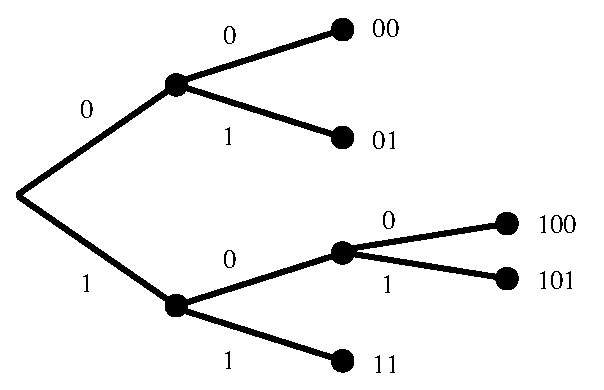
\epsfig{file=Figures/binarytreecode,width=7cm}
\end{psfrags}
\caption{Construction of a prefix code with a binary tree.}
\label{figure:BinaryTreeCode}
\end{center}
\end{figure}
\end{example}

Now that we know how to build instantaneous, we consider the problem of finding a prefix code with the smallest possible expected length.

\newpage

\begin{theorem}[Source-Coding Theorem]
Consider a discrete memoryless source $(\mathcal{X}, p_X(\cdot)$ and let $X$ be a random variable distributed according to $p_X (\cdot)$.
This source can be endoded with arbitrarily small error probability at any rate $R > H(X)$.
Conversely, if $R < H(X)$, the error will be non zero.
\end{theorem}


\section{Huffman Code}

\emph{Huffman coding} is a variable-length encoding algorithm used for lossless data compression.
The underlying strategy in this scheme is to assign short strings of bits to likely symbols, and longer ones to less probable source outputs.
The encoding is specifically crafted so that the code table forms a prefix code.
Huffman coding is the most efficient compression mapping for individual source simbols.
The expected length of the compressed data under this algorithm will be no greater than the expected message length of any other proper encoding scheme that operates on individual source symbols.



Although Huffman coding is optimal for a symbol-by-symbol encoding with a known input probability mass function, it can be outperformed when these two conditions are not known.
For instance, if the input distribution $p_x(\cdot)$ is not known, then it must be infered from the available data prior to applying Huffman coding.
Small errors in the estimated probability mass function can then lead to inefficiency, which in turn renders Huffman coding suboptimal.
More importantly, a more efficient way to encode data is to consider blocks of source symbols and to encode them jointly.
Although more complicated, this process leads to better performance and typically leads to expected message lengths that are lower than that of a typical symbol-by-symbol Huffman code.


\section{Lempel-Ziv Algorithm}

